%UNIT 1: QUALITATIVE AND GRAPHICAL APPROACHES
% Is first part of original 01.tex
%%%%%%%%%%%%%%%%%%%%%%%%%%%
%%%% Put the following at the top of each .tex file  %
\pagestyle{fancy}
\renewcommand{\theUnit}{2}
\ifthenelse{\isundefined{\UnitPageNumbers}}{}{\setcounter{page}{1}}
\rhead{Carlton and Devore Chapter \theUnit: Discrete Random Variables}
\lhead{Math 3382: Statistical Theory}
%\lhead{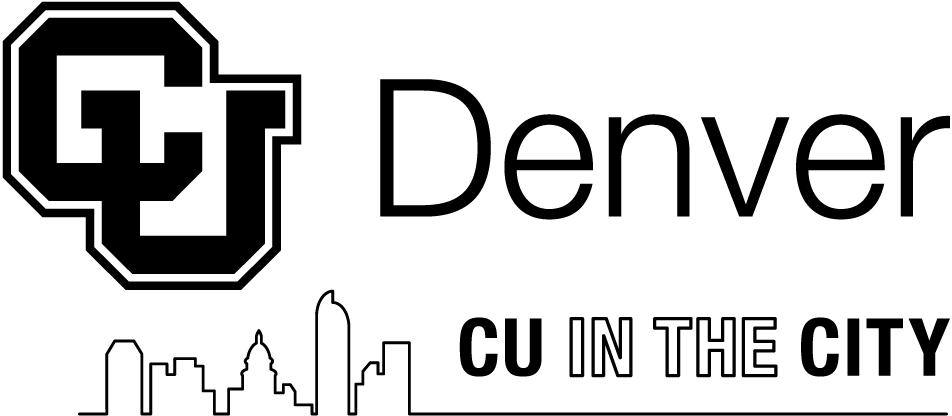
\includegraphics[width=1.25cm]{CUDenver-Logo.png}}
\rfoot{\mypage}
\cfoot{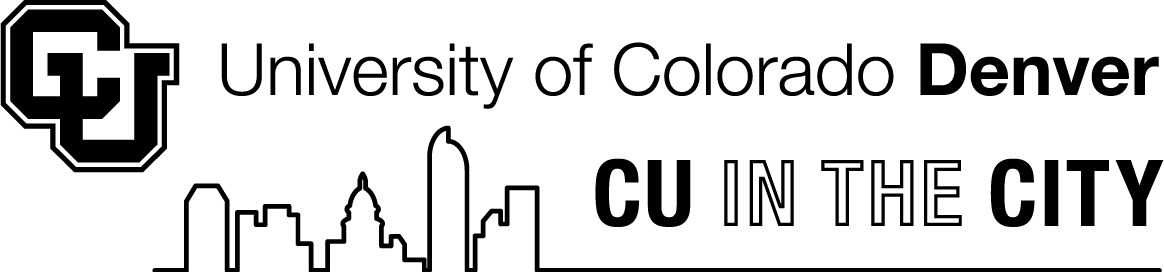
\includegraphics[width=2.25cm]{CUDenver-Logo-coverpage.png}}
\lfoot{Adam Spiegler}
\fancypagestyle{firstfooter}{\footskip = 50pt}
\renewcommand{\footrulewidth}{.4pt}
%%%%%%%%%%%%%%%%%%%%%%%%%%%
\vspace*{-20pt} \thispagestyle{firstfooter}

\pagebegin{Introduction to Random Variables}

Suppose a company knows that 1\% of the lithium batteries they manufacture are defective.  The manufacturer sends a shipment of 10 batteries to one of their clients. How likely is it that none of the batteries are defective? How can we connect the data to the concepts of sample spaces and events to answer this question? This link can be made using \textbf{\alert{random variables}}:

\begin{tcolorbox}
\begin{definition}\label{def:rv}
A \textbf{\alert{random variable}} is a mapping
\[ X: \Omega \to \mathbb{R} \]
that assigns a real number $X(\omega)$ to each outcome $\omega \in \Omega$.
\end{definition}
\end{tcolorbox}

For example, the random variable $X$ could map an outcome in which 10 batteries are selected at random to a number corresponding to how many batteries in the sample are not defective, denoted $G$ for good. For instance if $\omega = DDGGGGGGGG$, then $X(DDGGGGGGGG)=8$. We can calculate the probability that $X=10$ (none are defective) using independence of events:
\[ P(X=10) = P(G)P(G) \cdots P(G) = (P(G))^{10} = (0.99)^{10} \approx 0.9044.\]

\bb
\ii A student takes a 3 question quiz. Each of the 3 questions is multiple choice with 4 possible answer choices. Let the random variable $X$ be the number of correct guesses out of the 3 questions.\label{quiz}
\bb
\ii What is the sample space $\Omega$?\label{quizA}
\vspace{0.75in}
\ii Compute $P(X=0)$, how likely is it that the student gets none of the questions correct?
\vspace{0.75in}
\ii Fill in the empty entries in table below

\begin{center}
\begin{tabular}{|c|c|c|c|c|}
\hline
$x$ & \hspace{0.25in} 0  \hspace{0.25in} &  \hspace{0.25in} 1  \hspace{0.25in} &  \hspace{0.25in} 2  \hspace{0.25in} &  \hspace{0.25in} 3  \hspace{0.25in} \\
\hline
 & & & & \\
$P(X=x)$ & & & & \\
 & & & & \\
\hline
\end{tabular}
\end{center}

\ii Compute $P(X \leq 1)$ and interpret the practical meaning of this value.
\ee
\ee

\clearpage

\pagebegin{Distribution Functions}

\begin{tcolorbox}
\begin{definition}\label{def:pmf}
If $X$ is a \textbf{\alert{discrete}} random variable, we define the probability function or \textbf{\alert{probability distribution}} or \textbf{\alert{probability mass function (pmf)}}
for $X$ by
\[ p(x) = P(X=x) .\]
\end{definition}

\vspace{-0.25in}

\begin{definition}\label{def:cdf1}
If $X$ is a random variable, we define the \textbf{\alert{cumulative distribution function (cdf)}} as the function
\[ F(x)=P(X \leq x) = \sum_{k=\mbox{\scriptsize{min value}}}^x p(k) .\]
\end{definition}
\end{tcolorbox}

% Below is a geogebra interactive thing with binomial
% https://www.geogebra.org/m/GyYQWWNX

\bb[resume]
\ii Sketch the pmf and cdf for the random variable $X$ (number of correct guesses on the 3 question quiz) in question \ref{quiz}. Be sure to label the tickmarks on the vertical axes with an appropriate scale.

\begin{center}
\begin{tabular}{ll}
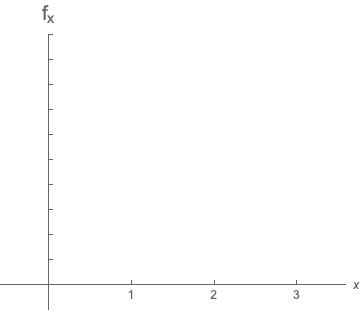
\includegraphics[width=0.3\tw]{04/04-blank-pmf.png} \hspace{1in} &
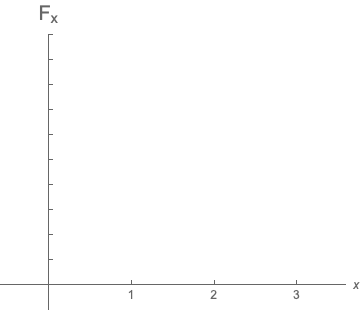
\includegraphics[width=0.3\tw]{04/04-blank-cdf.png} \\
Sketch the pmf, $p(x)$. & Sketch the cdf, $F(x)$\\
\end{tabular}
\end{center}

\ii Let $X$ is a discrete random variable with pmf and cdf denoted $p(x)$ and $F(x)$, respectively. Determine if each statement is True or False.
\begin{tasks}[counter-format = {(tsk[a])},label-offset = {0.8em},label-format = {\color{black}}](2)
\task $0 \leq p(x) \leq 1$ for all $x$.
\task $0 \leq F(x) \leq 1$ for all $x$. \vspace{0.45in}
\task $\dsty \sum_{\mbox{all $x$}} p(x) = 1$.
\task $\dsty \sum_{\mbox{all $x$}} F(x) = 1$. \vspace{0.45in}
\task $\dsty \lim_{x \to \infty} p(x) = 1$.
\task $\dsty \lim_{x \to \infty} F(x) = 1$. \vspace{0.45in}
\task The pmf must be a nondecreasing function.
\task The cdf must be a nondecreasing function. \vspace{0.45in}
\end{tasks}
\ee

\clearpage

\pagebegin{Expected Value and Variance}

\begin{tcolorbox}
\begin{definition}\label{def:expected}
The average or \textbf{\alert{expected value}} for a discrete random variable $X$ is denote $E(X)$ or $\mu$ and computed using the formula
\[ E(X) = \mu =  \sum_x \left( x \cdot p(x) \right) = \sum_x \left( x \cdot P(X=x) \right). \]
\end{definition}
\vspace{-0.5in}

\begin{definition}\label{def:variance}
The \textbf{\alert{variance}} for a discrete random variable $X$ is one common way to measure how spread out (in relation to the expected value) are the values of $X$. The variance is denoted $\Var(X)$ or $\sigma^2$ and computed using the formula
\[ \Var(X) = \sigma^2 =  \sum_x \left( (x-\mu)^2 \cdot p(x) \right) = \sum_x \left( (x-\mu)^2 \cdot P(X=x) \right). \]
\end{definition}
\vspace{-0.5in}

\begin{definition}\label{def:variance}
The \textbf{\alert{standard deviation}} for a discrete random variable $X$ is the square root of the variance and is denoted by $\sigma$. It more or less measures the average of the distances for each value of $X$ from the mean $\mu$.
\[ \mbox{SD}(X) = \sigma =  \sqrt{\Var(X)}. \]
\end{definition}


\end{tcolorbox}

\bb[resume]
\ii Using properties of the pmf, $p(x)$, show that \label{var-prop}
\begin{tcolorbox}
\[ \Var(X) = E(X^2)  - \mu^2  \]
\end{tcolorbox}

\vspace{0.5in}
\vfill

\ii A charity is running a raffle as afundraiser. They offer one grand prize of \$$500$, two second prizes of \$$100$ each, and ten third prizes of \$$20$ each. They plan to sell $1,\!000$ tickets each at a price of \$$2$. Let $X$ denote the amount of money won by a lottery ticket.\label{lottery}
\bb
\ii Fill in the values of $x$ and $p(x)$ in the table below.\medskip

\begin{center}
\begin{tabular}{|c||c|c|c|c|}
\hline
$x$ &  \hspace{0.5in}  &  \hspace{0.5in}  &  \hspace{0.5in}  &  \hspace{0.5in} \\
\hline
$p(x)$ & & & &  \\
\hline
\end{tabular}
\end{center} \medskip
%\begin{center}
%\begin{tabular}{c|c|c}
%x & \hspace{0.5in} P(x) \hspace{0.5in} & \hspace{1in} $(x-\mu)^2$ \hspace{1in}  \\
%\hline
 % & & \\
 %   & & \\
%\hline
%  & & \\
 %   & & \\
%\hline
%  & & \\
 %   & & \\
%\hline
%  & & \\
 %   & & \\
%\end{tabular}
%\end{center}  \medskip

\ii Calculate $E(X)$ and $\Var(X)$.
\ee
\ee
\vfill
